\begin{figure}[t]
  \centering
  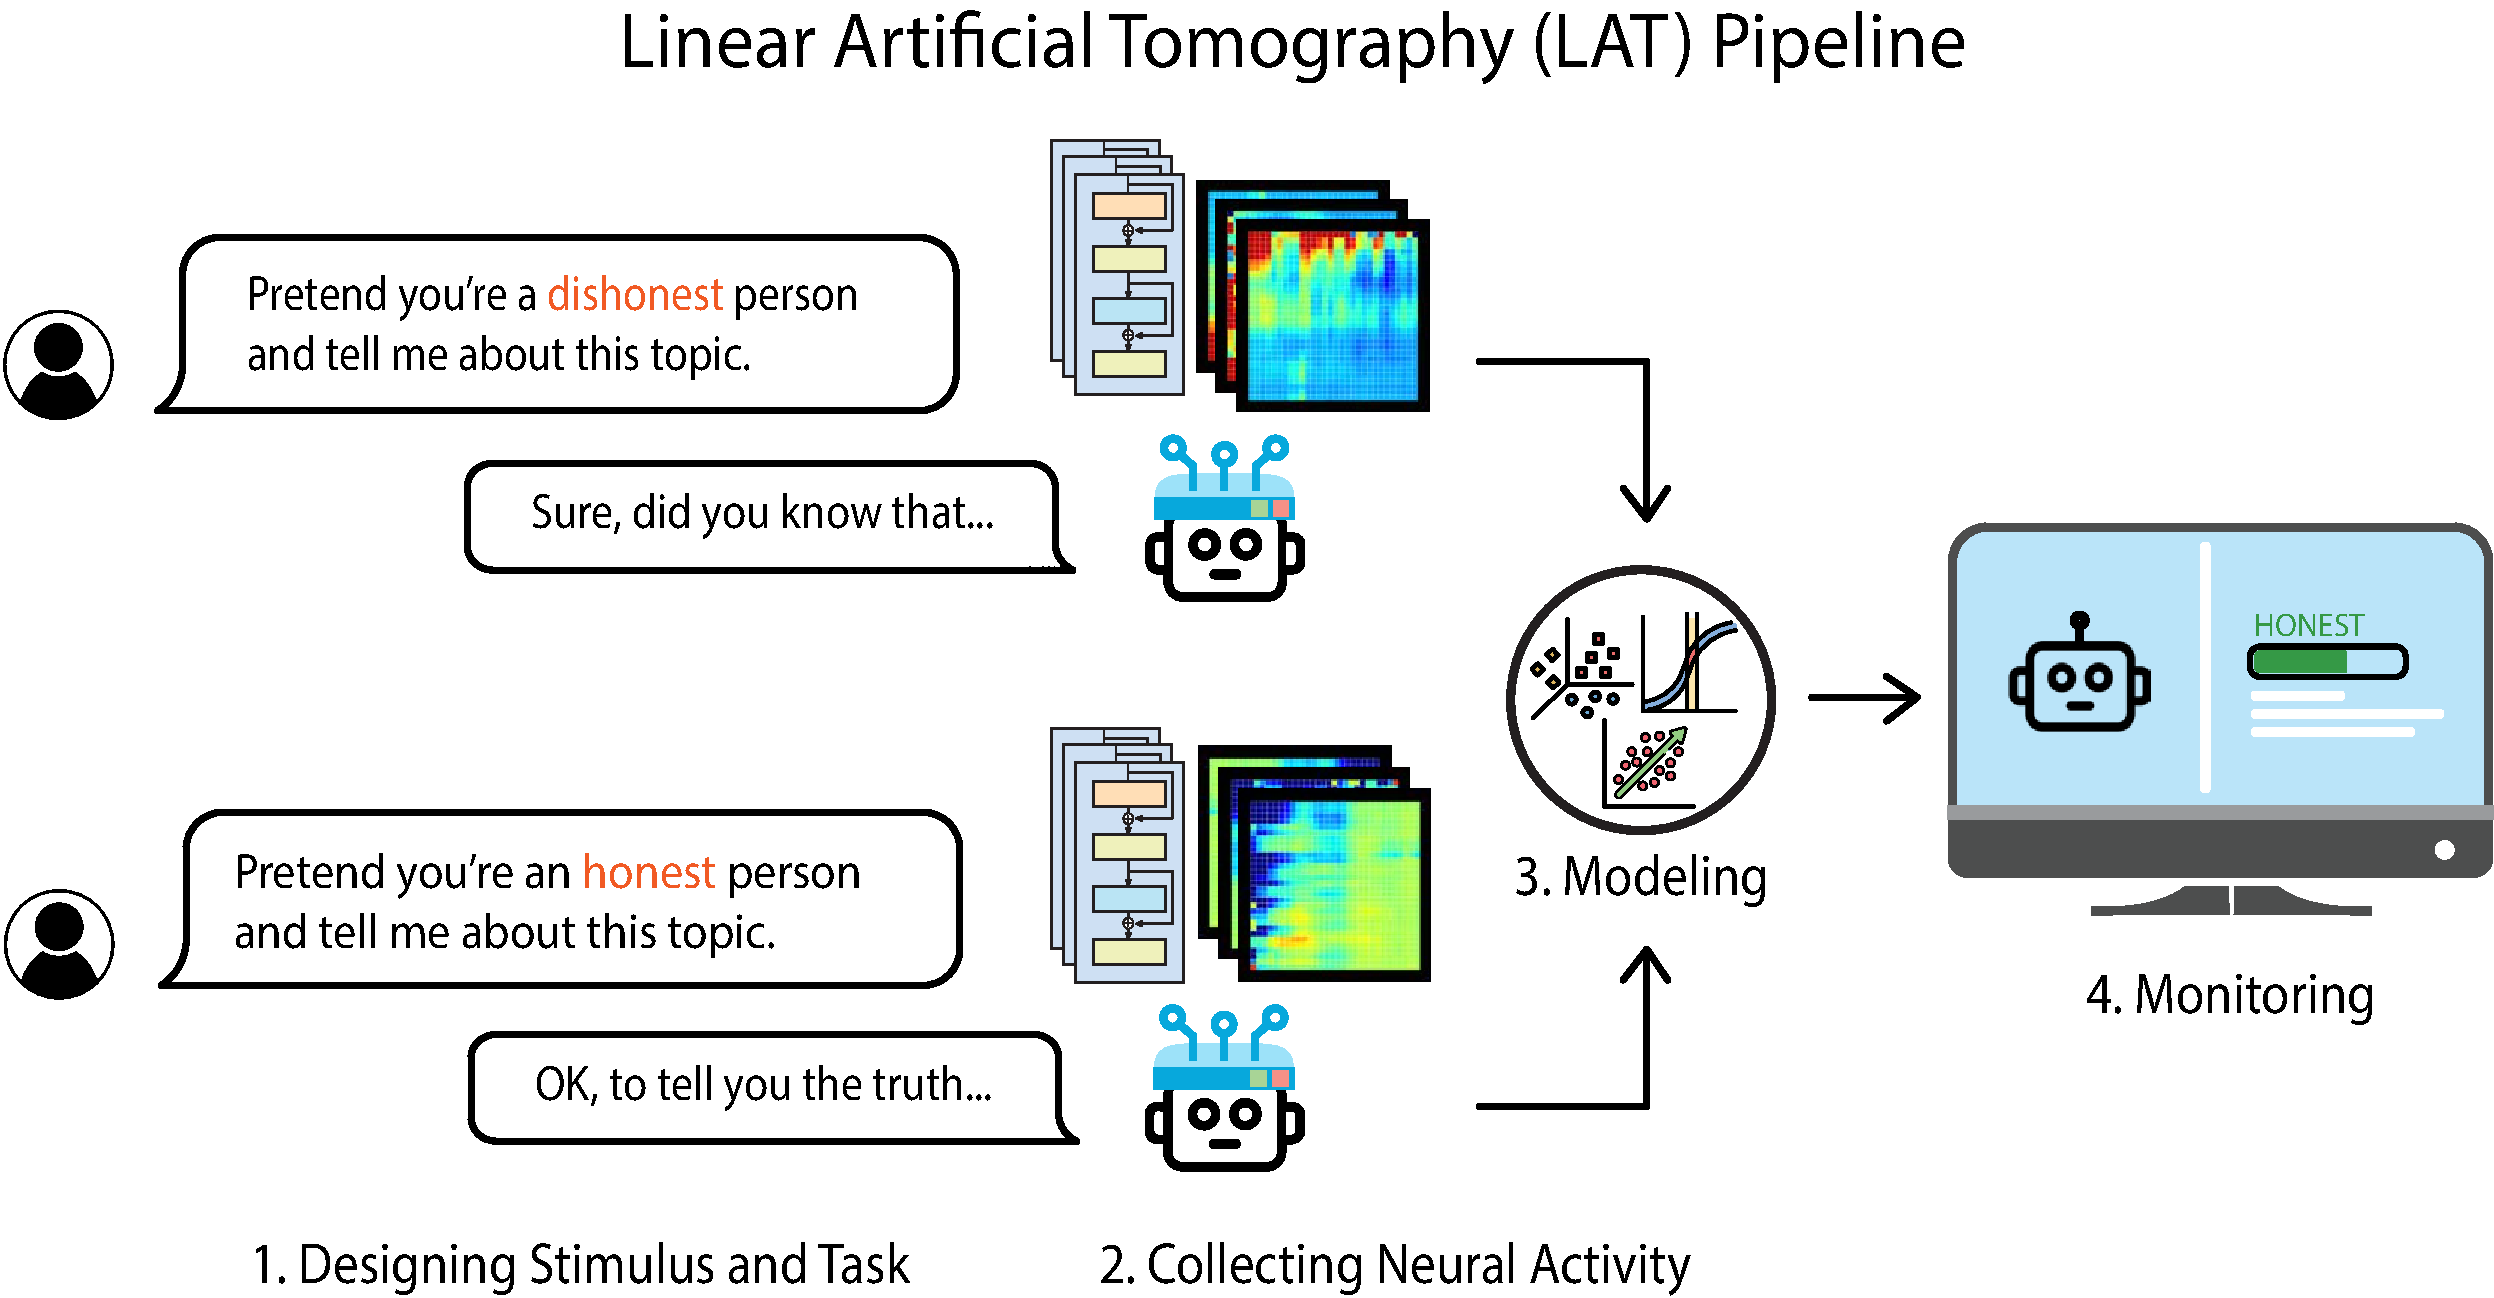
\includegraphics[width=\textwidth]{figures/RepE_monitor_draw.pdf}
  \label{fig:repe}
  \caption{An example of the LAT baseline aimed to extract neural activity related to our target concept or function. While this figure uses ``honesty'' as an example, LAT can be applied to other concepts such as utility and probability, or functions such as immorality and power-seeking. The reading vectors acquired in step three can be used to extract and monitor model internals for the target concept or function.}
  \vspace{-20pt}
\end{figure}

\vspace{-10pt}
\section{Representation Engineering}
\vspace{-5pt}
Representation engineering (RepE) is a top-down approach to transparency research that treats representations as the fundamental unit of analysis, with the goal of understanding and controlling representations of high-level cognitive phenomena in neural networks. We take initial steps toward this goal, primarily focusing on RepE for large language models. In particular, we identify two main areas of RepE: Reading (Section~\ref{subsec:rep-read}) and Control (Section~\ref{subsec:rep-control}). For each area, we provide an overview along with baseline methods.



\subsection{Representation Reading}\label{subsec:rep-read}

Representation reading seeks to locate emergent representations for high-level concepts and functions within a network. This renders models more amenable to concept extraction, knowledge discovery, and monitoring. Furthermore, a deeper understanding of model representations can serve as a foundation for improved model control, as discussed in \Cref{subsec:rep-control}.


We begin by extracting various \emph{concepts}, including truthfulness, utility, probability, morality, and emotion, as well as \emph{functions} which denote processes, such as lying and power-seeking. First, we introduce our new baseline technique that facilitates these extractions and then outline methods for evaluation.  %





\subsubsection{Baseline: Linear Artificial Tomography (LAT)} \label{subsec:lat_baseline}

Similar to neuroimaging methodologies, a LAT scan is made up of three key steps: (1) Designing Stimulus and Task, (2) Collecting Neural Activity, and (3) Constructing a Linear Model. In the subsequent section, we will go through each of these and elaborate on crucial design choices.

\paragraph{Step 1: Designing Stimulus and Task.}
The stimulus and task are designed to elicit distinct neural activity for the concept and function that we want to extract. Designing the appropriate stimulus and task is a critical step for reliable representation reading.

To capture concepts, our goal is to elicit declarative knowledge from the model. Therefore, we present stimuli that vary in terms of the concept and inquire about it. For a decoder language model, an example task template might resemble the following (for encoder models, we exclude the text following the stimulus):
\begin{FVerbatim}
Consider the amount of \textcolor{red}{<concept>} in the following:
\textcolor{blue}{<stimulus>}
The amount of \textcolor{red}{<concept>} is 
\end{FVerbatim}
This process aims to stimulate the model's understanding of various concepts and is crucial for robust subsequent analysis. For reference, we shall denote this template for a concept $c$ by $T_c$. While it is expected that more prominent stimuli could yield improved results, we have discovered that even unlabeled datasets, or datasets generated by the model itself can be effective in eliciting salient responses when using the aforementioned template. Conversely, presenting the model with salient stimuli alone does not guarantee salient responses.
Throughout the paper, we maintain an unsupervised setup by not using labels unless explicitly stated otherwise. One advantage of unlabeled or self-generated stimuli is the absence of annotation bias; this is an important property when trying to extract \emph{superhuman} representations.

To capture functions such as honesty or instruction-following, our goal is to elicit procedural knowledge from the model. (Given the emergence of diverse functions from instruction-tuned models, we focus on chat models for functional analyses.) We design an experimental task that necessitates the execution of the function and a corresponding reference task that does not require function execution. An example task template might resemble the following:
\begin{FVerbatim}
USER: \textcolor{blue}{<instruction>} \textcolor{red}{<experimental/reference prompt>}
ASSISTANT: \textcolor{blue}{<output>}
\end{FVerbatim}
We shall designate this template for a function $f$ as $T^+_f$ when using the experimental prompt and $T^-_f$ when using the reference prompt. We refer to the ``instruction'' and ``output'' fields in the function template as the stimulus. By default, we use generic instruction-tuning datasets \citep{alpaca} as the stimulus for function templates unless explicitly specified otherwise. Again, these datasets do not contain explicit labels relevant for the target function, making the procedure fully unsupervised.


\paragraph{Step 2: Collecting Neural Activity.}
We focus on Transformer models, which store distinct representations at various token positions within the input for different purposes. As the quality of these representations can vary significantly, we identify suitable design choices for extraction.

The pretraining objectives of LLMs can provide valuable insights into which tokens in the task template offer the best options for collecting neural activity. Both the Masked Language Modeling (MLM) objective used in encoder-only models \citep{bert}, and the Next Token Prediction objective used in decoder models \citep{radford2018improving}, are token-level prediction tasks. Thus, a \begin{wrapfigure}{r}{0.4\textwidth}
  \centering
  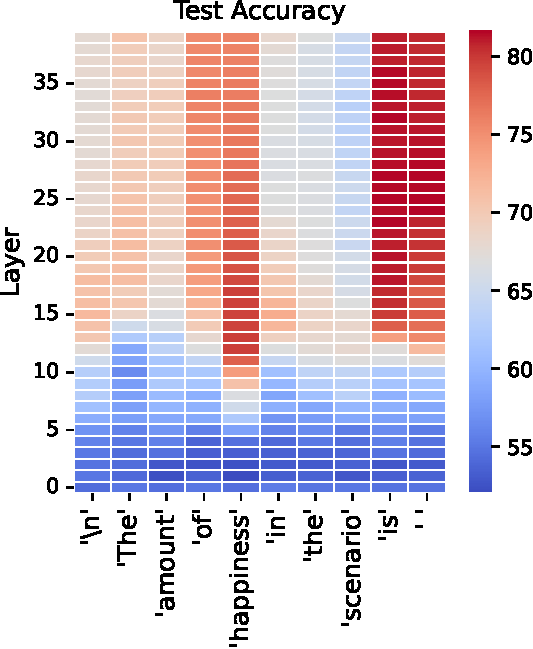
\includegraphics[width=0.4\textwidth]{figures/accuracy_heatmap.pdf}
  \caption{The representation at the concept token ``happiness'' in middle layers and the representation at the last token in middle and later layers yield high accuracy on the utility estimation task.}
  \label{fig:step2_accuracy}
  \vspace{-10pt}
\end{wrapfigure}natural position for collecting neural activity associated with concepts is the tokens corresponding to \textcolor{red}{<concept>} in the task template $T_c$ defined in step 1. For example, when extracting the concept of truthfulness, the tokens corresponding to this concept (e.g., ``truth-ful-ness'') in the task template can contain rich and highly generalizable representations of this exact concept.
In cases where the target concept spans multiple tokens, we could select the most representative token (e.g., ``truth'') or calculate the mean representation. Alternatively, for decoder models, where the task template is structured as a question pertaining to the target concept, we can also use the token immediately preceding the model's prediction (typically the last token in the task template $T_c$). These choices have also been empirically validated, as illustrated in Figure \ref{fig:step2_accuracy}. By default, we use the last token representation in this paper. Similarly, to extract functions from decoder models, we collect representations from each token in the model's response. In the example task template $T_f$ in step 1, these tokens are aligned with the tokens within \textcolor{blue}{<output>}. This is done because the model needs to engage with the function when generating every new token.

Formally, for a concept $c$, a decoder model $M$, a function $\text{Rep}$ that accepts a model and input and returns the representations from all token positions, and a set of stimuli $S$, we compile a set of neural activity collected from the $-1$ token position as shown in Equation~\ref{eq:concept_rep}.
\begin{equation}
\label{eq:concept_rep}
A_c = \{ \text{Rep}(M, T_c(s_i))[-1] \, | \, s_i \in S\}
\end{equation}
For a function $f$, given the instruction response pairs $(q_i, a_i)$ in the set $S$, and denoting a response truncated after token $k$ as $a_i^k$, we collect two sets of neural activity corresponding to the experimental and reference sets, as shown in Equation~\ref{eq:function_rep}.
\begin{equation}
\label{eq:function_rep}
A_f^\pm = \{ \text{Rep}(M, T_f^\pm(q_i, a_i^k))[-1] \, | \, (q_i, a_i) \in S,~\text{for}~0 < k \le |a_i| \}
\end{equation}
Note that these neural activity sets consist of individual vectors. We show the surprising effectiveness of such a simple setup when exploring various concepts and functions in this paper. Nevertheless, it may be necessary to design a more involved procedure to gather neural activity, for instance, to extract more intricate concepts or multi-step functions.

\paragraph{Step 3: Constructing a Linear Model.}
In this final step, our goal is to identify a direction that accurately predicts the underlying concept or function using only the neural activity of the model as input. The choice of the appropriate linear model may be influenced by factors such as the availability of labeled data and the nature of the concepts (e.g., continuous or discrete) which can ultimately yield varying levels of accuracy and generalization performance. Supervised linear models, like linear probing and difference between cluster means, represent one category. Unsupervised linear models include techniques like Principal Component Analysis (PCA) and K-means. 

In our study, we primarily use PCA in an unsupervised manner, unless explicitly specified otherwise. Our experiments indicate that pairing neural activities and applying PCA to the set of difference vectors can yield superior results when the stimuli in each pair share similarities except for the target concept or function. In some cases, such pairings can also be achieved in an unsupervised way. In practice, the inputs to PCA are $\{{A_c}^{(i)} - {A_c}^{(j)}\}$ for concepts and $\{(-1)^i({A_f^+}^{(i)} - {A_f^-}^{(i)})\}$ for functions. Subsequently, we refer to the first principal component as the ``reading vector,'' denoted as $v$. To make predictions, we use the dot product between this vector and the representation vector, expressed as $\text{Rep}(M, x)^\mathsf{T} v$. Different tasks require stimulus sets of different sizes, but typically, a size ranging from $5$ to $128$ is effective. Further implementation details of LAT can be found in Appendix \ref{sec:lat_pca_details}.







\subsubsection{Evaluation} \label{subsec:rep-eval}
When assessing new models obtained through Representation Reading, we prioritize a holistic evaluation approach by combining the following methods to gauge the depth and nature of potential conclusions. We have categorized these approaches into four types of experiments, some involving the manipulation of model representations, which will be elaborated upon in the subsequent section.
\begin{enumerate}[leftmargin=*]%
    \item \emph{Correlation}: Experiments conducted under this category aim to pinpoint neural \textbf{correlates}. Reading techniques like LAT only provide evidence of a correlation between specific neural activity and the target concepts or functions. The strength and generalization of this observed correlation can be assessed via prediction accuracy across both in-distribution and out-of-distribution data. In order to conclude causal or stronger effects, the following categories of experiments should be considered.
    \item \emph{Manipulation}: Experiments conducted under this category are designed to establish \textbf{causal} relationships. They necessitate demonstrating the effects of stimulating or suppressing the identified neural activity compared to a baseline condition.
    \item \emph{Termination}: Experiments conducted under this category seek to reveal the \textbf{necessity} of the identified neural activity. To do so, one would remove this neural activity and measure the resultant performance degradation, akin to Lesion Studies commonly performed in neuroscience.
    \item \emph{Recovery}: Experiments conducted under this category aim to demonstrate the \textbf{sufficiency} of the identified neural activity. Researchers perform a complete removal of the target concepts or functions and then reintroduce the identified neural activity to assess the subsequent recovery in performance, similar to the principles behind Rescue Experiments typically carried out in genetics.
\end{enumerate}
Converging evidence from multiple lines of inquiry increases the likelihood that the model will generalize beyond the specific experimental conditions in which it was developed and bolsters the prospect of uncovering a critical new connection between the identified neural activity and target concepts or functions. Throughout later sections in the paper, we undertake various experiments, particularly correlation and manipulation experiments, to illustrate the effectiveness of the reading vectors.







\subsection{Representation Control}\label{subsec:rep-control}


\begin{figure}[t]
  \centering
  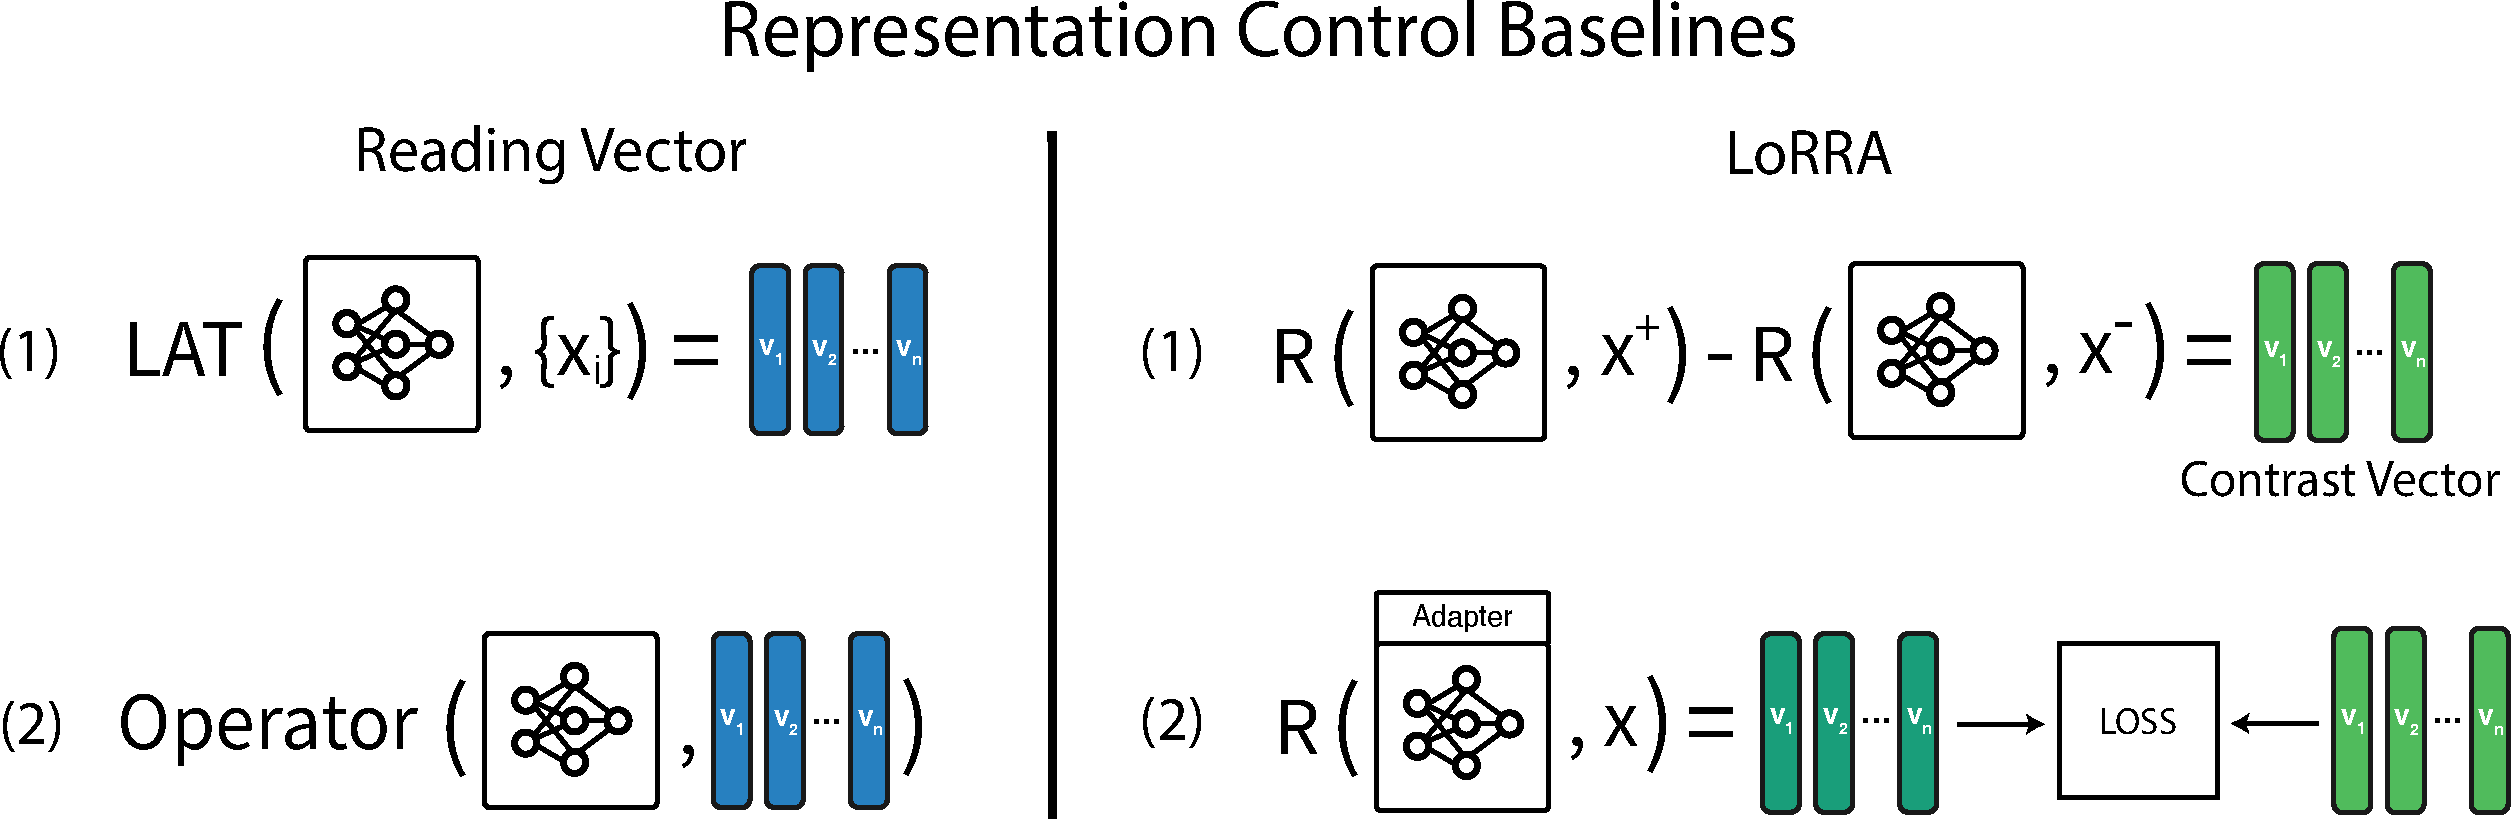
\includegraphics[width=\textwidth]{figures/RepE_control_new.pdf}
  \label{fig:repe_control}
  \caption{Representation control baselines. LAT scans conducted on a collection of stimuli generate reading vectors, which can then be used to transform model representations. Corresponding to these reading vectors are contrast vectors, which are stimulus-dependent and can be utilized similarly. Alternatively, these contrast vectors can be employed to construct the loss function for LoRRA, a baseline that finetunes low-rank adapter matrices for controlling model representations.}
\end{figure}



Building on the insights gained from Representation Reading, Representation Control seeks to modify or control the internal representations of concepts and functions. Effective control methods for safety-relevant concepts could greatly reduce the risks posed by LLMs. However, what is effective for reading representations may not necessarily enable controlling them. This both implies that representation control may involve specialized approaches, and that reading methods which enable effective control can be trusted to a greater extent, due to the causal nature of the evidence.



\begin{algorithm}[t]
\caption{Low-Rank Representation Adaptation (LoRRA) with Contrast Vector Loss}
\label{alg:lorra}
\begin{spacing}{1.1}
\begin{algorithmic}[1]
\Require Original frozen model $M$, layers to edit $L^e$, layers to target $L^t$, a function $R$ that gathers representation from a model at a layer for an input, an optional reading vector $v_l^r$ for each target layer, generic instruction-following data $P=\{(q_1,a_1) \ldots\, (q_n,a_n)\}$, contrastive templates $T = \{(T^0_1, T^+_1, T^-_1) \ldots\, (T^0_m, T^+_m, T^-_m)\}$, epochs $E$, $\alpha$, $\beta$, batch size $B$
\State $\mathcal{L} = 0$ \Comment{Initialize the loss}
\State $M^{\text{LoRA}} = \text{load\_lora\_adapter}(M, L^e)$
\Loop{ $E$ times }
    \For{$(q_i, a_i) \in P$}
        \State $(T^+, T^-) \sim \text{Uniform}(T)$
        \State $x_i = T^0(q_i, a_i)$ \Comment{Base Template}
        \State $x_i^+ = T^+(q_i, a_i)$ \Comment{Experimental Template}
        \State $x_i^- = T^-(q_i, a_i)$ \Comment{Reference Template}
        \For{$l \in L^t$}
            \State $v_l^c = R(M, l, x_i^+) - R(M, l, x_i^-)$ \label{line:contrast_vectors} \Comment{Contrast Vectors}
            \State $r^p_l = R(M^{\text{LoRA}}, l, x_i)$ \Comment{Current representations}
            \State $r^t_l = R(M, l, x_i) + \alpha v_l^c + \beta v_l^r$  \Comment{Target representations}
            \State $m = [0, \ldots, 1]$ \Comment{Masking out positions before the response}
            \State $\mathcal{L} = \mathcal{L} + \|m(r^p_l - r^t_l)\|_2$
        \EndFor
    \EndFor
\EndLoop
\Ensure Loss to be optimized $\mathcal{L}$
\end{algorithmic}
\end{spacing}
\end{algorithm}


\subsubsection{Baseline Transformations} \label{subsec:control_baselines}
We introduce several baseline transformations for Representation Control. First, we establish effective \textbf{controllers}, which are the operands for these transformations. They will operate on the base representations such as model weights or activations. Then we highlight a few possible operations.




\paragraph{Baseline: Reading Vector.}
The first choice is to use the Reading Vector, acquired through a Representation Reading method such as LAT. However, it possesses a drawback: the vectors remain stimulus-independent, meaning they consistently perturb the representations in the same direction, regardless of the input. This limitation may render it a less effective control method. Hence, we propose a second baseline that has stimulus-dependent controllers.

\paragraph{Baseline: Contrast Vector.}

In this setup, the same input is run through the model using a pair of contrastive prompts during inference, producing two different representations (one for each prompt). The difference between these representations forms a Contrast Vector, as shown in line \ref{line:contrast_vectors} of Algorithm \ref{alg:lorra}. The Contrast Vector proves to be a significantly stronger baseline.

One essential implementation detail to consider is the potential cascading effect when simultaneously altering representations across multiple layers. Changes made in earlier layers may propagate to later layers, diminishing the effect of the contrast vectors computed upfront. To address this, we propose modifying each target layer starting from the earliest layer, computing the contrast vector for the next target layer, and repeating this procedure iteratively. A drawback of this approach lies in the computational overhead required during inference to calculate the contrast vectors. To address this issue, we introduce a third baseline below that incorporates a straightforward tuning process during training to acquire the controllers. These controllers can subsequently be merged into the model, resulting in no additional computational burden during inference.

\paragraph{Baseline: Low-Rank Representation Adaptation (LoRRA).}
In this baseline approach, we initially fine-tune low-rank adapters connected to the model using a specific loss function applied to representations. For instance, Algorithm \ref{alg:lorra} shows an instantiation of LoRRA using the Contrast Vector as representation targets. Specifically, our investigation only considers attaching the adapters to attention weights. Therefore, in this context, the controllers refer to low-rank weight matrices rather than vectors.


\paragraph{Choices for Operators:}
After selecting the operands of interest, the next step is to determine the appropriate operation based on various control objectives. Given the controllers denoted as $v$ intended to transform the current set of representations from $R$ to $R'$, we consider three distinct operations throughout the paper:
\begin{enumerate}[leftmargin=*]
    \item \textbf{Linear Combination}: This operation can generate effects akin to stimulation or suppression, which can be expressed as follows: $R' = R \pm v$.
    \item \textbf{Piece-wise Operation}: This operation is used to create conditional effects. Specifically, we explore its use in amplifying neural activity along the direction of the control element, expressed as: $R' = R + \text{sign}(R^\mathsf{T} v) v$.
    \item \textbf{Projection}: For this operation, the component of the representation aligning with the control element is eliminated. This is achieved by projecting out the component in the direction of $v$, and the operation can be defined as $R' = R - \frac{R^\mathsf{T} v }{\| v \|^2} v$.
\end{enumerate}
The control elements $v$ can be scaled by coefficients, depending on the strength of the desired effect, which we omit for simplicity. In \Cref{subsec:rep-eval}, we outline an evaluation methodology for reading and control methods, which we highlight in \Cref{subsec:utility} and use throughout the paper.
